\section{Results}

\subsection{Multi-wavelength single-molecule co-localization methods}

Before describing the approach used for the analysis of CoSMoS data, it is helpful to  review briefly the experimental method. A representative CoSMoS experiment is illustrated by the example in Figure~1. The key features of a CoSMoS experiment include: 1) One species of fluorescently labeled molecule (called the “target”) is tethered to the surface of the observation chamber. Target molecules are immobilized at a surface density sufficiently low that the mean nearest-neighbor distance is large relative to the point-spread function (i.e., the diffraction-limited spot size) of the microscope. 2) Molecules, each species labeled with a different dye color, are added to the solution over the surface, typically at concentrations $\leq 1 \mu$M. When these “binder” molecules are freely diffusing in solution, they are invisible in TIRF. In contrast, when they are bound to the target, single binder molecules are detected as discrete fluorescent spots. The combination of features 1 and 2 means that formation of an individual binder-target complex is detected as spot appearance; dissociation of a binder-target complex is detected as spot disappearance \cite{Friedman2006-kb, Friedman2015-nx}.

\subsection{CoSMoS image data}

Preprocessing of CoSMoS data includes localization of target molecules in the target channel, registration of target and binder channels, and time-dependent drift correction \cite{Friedman2015-nx, Smith2019-yb} (Figure 1B). After preprocessing data consists of a time series of squares of images confined to the area of interest (AOI) centered at each target molecule. The size of the AOI has to be large enough so that on-target spot can be clearly distinguished from background and  reliably  determine  the  local  background  intensity. Based on the typical half-width of 1-2 pixels for fluorescent spots we chose conservatively the size of AOI to be 14x14 pixels (Figure 1C).

Frequently, identification of on-target binding is complicated by molecules binding off-target which distort the shape of the on-target spot and its apparent distance to the target. In addition to the on-target spot, non-specifically bound binder molecules can also be present in the image. Unlike on-target binding, nonspecific interaction can be anywhere in the image. We explicitly model these nonspecific binding events. Usually no more than two spots are present in the single image. Optionally, off-target control data is also constructed from randomly selected sites at which no target molecule is present. Off-target control data helps to constraint the frequency of nonspecific binding (Figure 1D). % One experiment typically consists of a set of images where we have $N$ target sites ($n \in \{1,\dots,N\}$) each consisting of a series of $F$ different images in a recording ($f \in \{1,\dots,F\}$) (a “recording”).

\subsection{Overview}

The most basic task in CoSMoS data analysis is spot discrimination. The goal is to acquire information at each time point about whether a binder molecule fluorescence spot is observed at the image position of a target molecule (e.g., whether a co-localized green RNA polymerase is observed at the surface location of a blue DNA spot in Figure 1). To maximize the extraction of useful information from data we use full 2-D images for analysis. We analyze the images within Bayesian framework which requires choosing a probabilistic model for the observed data. In the Bayesian framework inference of model parameters (posterior distributions) is performed by using the Bayes' rule. We approximate diffraction-limited spots with 2-D Gaussians and use realistic intensity-dependent noise model. Bayesian modeling requires specification of priors which allows us to embed our knowledge about the experiment (e.g., the likely positions of an on-target and an off-target spots). Our approach in this work  is “time-independent” meaning that we ignore the time dimension of the recording -- the order of the images is arbitrary and does not affect the model, as each image is considered statistically independent of the others. The model and the inference of model parameters were implemented as a probabilistic program, Tapqir, in the Python-based probabilistic programming language (PPL) Pyro. % To analyze the CoSMoS image classification problem within Bayesian framework, one must choose a probabilistic model for the observed data, formalized in a likelihood function. 

\subsection{Image Model} 

The simplest CoSMoS data set consists of a set of images (a “recording”) where each image is represented as a matrix of pixel intensity values (Figure 2A). In each image, a binder molecule is either present on the single target molecule or absent. We model the observed data as a mixture distribution of  as “spot” images of binder molecules superimposed on background image. We explicitly models both on-target and off-target spots. Our model assumes that at maximum $K=2$ number of spots can be present in a single image. We use binary indicator variable $\mathbf{m} = \{\mathrm{m}_{nfk}\}$ to denote the presence of each individual spot ($k \in \{1,\dots,K\}$). There are four possible combinations of $m_1$ and $m_2$: (1) “no-spot” image that contain only background (Figure 2B top left), (2) single “spot” image that contain the first binder molecule spot superimposed on background (Figure 2B bottom left), (3) single “spot” image that contain the second binder molecule spot superimposed on background (Figure 2B top right), and (4) two spot image that contains two binder molecule spots superimposed on background that can vary from image to image (Figure 2B bottom right).  Noiseless background images consist of constant average background intensity $b$. Fluorescence spot is modeled as a 2D Gaussian which accurately approximates fluorescence microscope point spread function \cite{Zhang2007-rb}. Each spot is parameterized by integrated scalar intensity $\mathrm{h}_{nfk}$, width $\mathrm{w}_{nfk}$, and relative position $\mathrm{x}_{nfk}$ and $\mathrm{y}_{nfk}$ to the target molecule. All of the spot parameters are local/individual for each spot. % We assume that background and spots have Gaussian noise. (Improvement of the preliminary method to include more realistic noise models is proposed in Aim 1a.)  each spot image is modelled as a Gaussian perturbation of the sum of the background λae treat the image recording using a standard likelihood “mixture model”71, in which the data are considered a mixture of spot and background images of unknown proportions

\subsection{Co-localization}

For the spots that are present in the image they can be further classified as on-target (co-localization) or off-target (non-specific). The model assumes that at maximum only one on-target spot can be present in the single image. The value of the index variable $\theta_{nf} \in \{0,1,\dots,K\}$ specifies the index of the on-target spot when it is present (Figure 2D, mid and right) and equals zero when the on-target spot is absent (Figure 2D, left). Thus, there are total $2^K + K2^{K-1}$ unique combinations of $\mathrm{m}$ and $\theta$ which define the state space for mixture model. The probability of being on-target or off-target is dictated primarily by the distance to the target. Spots bound on-target and off-target have different prior distributions of their location relative to the target molecule. This prior knowledge is used to discriminate between on- and off-target spots in a probabilistic manner using mixture distributions model. Off-target spots have a uniform prior distribution across the image and can bind anywhere on the surface with equal probability. On-target spots, on the other hand, are clustered near the target molecule (Supplementary Figure 2). Standard deviation of the distribution of on-target spots depends on the spot localization accuracy and the mapping accuracy between target and binder channels (?). Second, the posterior probabilities of being classified as on-target or off-target spot depends on the prior average frequencies of on-target and off-target spots. Increasing the ratio of the off-target molecules to on-target molecules decreases the probability of the spot being on-target reflecting the fact that.

\subsection{Generative model}

We build a probabilistic model for CoSMoS data by introducing latent variables that explain how the observed data is generated. The probabilistic model can be interpreted as a generative process that produces the observed image data. A graphical model describing the probabilistic relationships in the model is shown in Figure 2C. In this directed graph, nodes are either random variables (circles) or deterministic functions (diamonds). Related nodes are connected by edges, with an arrow pointing towards the dependent variable. Dashed boxes represent activation of variables. Finally, plates represent replication and specify an index for the repeated variable. As was mentioned above, frames are treated as being time-independent. The image model described above allows to capture many of the characteristics of real experimental data, such as site and time dependent fluctuations in the local background signal, time dependent fluctuations in the spot intensity and its position, simultaneous binding of on-target and off-target spots, Gamma distributed noise, which is more realistic than Gaussian noise.

Total observed intensity is the sum of the offset signal (dark current) plus the photon counts amplified by the gain setting of the camera. The linear relationship between the noise variance and the mean intensity is built into the intensity model through the gain and offset parameters and the gain parameter is fitted along with other parameters. Distribution of the offset signal is obtained as a histogram density signal from the single-molecule images.

\subsection{Bayesian Inference and Implementation}

Posterior distributions of latent variables conditioned on the observed data is given by the Bayes' theorem. The evidence in general is intractable. Here we use stochastic variational inference (SVI) approach and maximize the evidence-lower bound (ELBO). Our program Tapqir is open-source (github link) and is implemented in the probabilistic programming language Pyro. The advantage of using PPL like Pyro is its black box SVI approach which allows to focus on the model, efficient computation on GPU, scalability to large datasets. Details of the generative model and variational model are given in the online Methods section.

\subsection{Figure 3. Tapqir analysis}

We demonstrate the application of Tapqir analysis on simulated and experimental data. (Generation of simulated and experimental data are explained in Methods). Analysis jointly fits on-target and control data. The algorithm produces a robust, statistics-based estimate of the probability that an on-target spot is present in each frame of the recording at every target molecule location. In addition, it provides posterior distributions for all model parameters from which mean values and confidence intervals can be calculated. Short extract of analysis results are shown for simulated data in Figure 3A and experimental data in Figure 3B. The program correctly detects spots both in simulated and experimental data. (Images) The program arbitrarily assigns spot 1 and spot 2 designations to features in the image. From p(m) and p(theta) the program calculates p. The algorithm recognizes the presence of on-target spots (p, green curve, e.g. frame 170 in A and frame 635 in B). The algorithm recognizes the presence of off-target spots (p, red curve, e.g. frame 173 in A and frame 635 in B). The program determines spot intensity and its position. Expectedly, there is a high uncertainty in the position of a spot when intensity is low (h, x, y). The program determines background intensity without requiring a separate measurement (b) (change the color). Talk about the possibility of spots being partially present for the duration of a single frame in experimental data

\subsection{Figure 4. Tapqir performance on simulated data}

As a validation of our model we demonstrate its application to simulated synthetic data. Fake-data simulation is important because it allows to directly check that the inference on latent variables is reliable. Thus, fake-data simulation provides an upper bound of what can be learned reliably about the model for various types of data. Simulation parameters details are described in the online Methods. We made 10 randomized simulations and then fit the synthetic data to the model. Figure 3 shows plots of the simulated values of the global parameters (gain, average on-target spot probability, average off-target spot probability, proximity) vs the fitted values. The results demonstrate that model parameters can be reliably recovered which is good.

By analyzing simulated data we have established that this parameter, also called the proximity parameter, can be reliably determined by floating it during the fit (Figure ). Alternatively, proximity parameter can be determined experimentally and fixed in the model. Figure show the distribution of the center of mass of on-target spots which are tightly clustered around the target molecule. On the other hand, off-target spots are distributed more uniformly across the area of the image.

This standard distribution can be determined independently and used as a fixed parameter in the model. However, it can also be floated in the fit and determined from the overall distribution of the center of masses of spots. $\sigma^{xy}$, $\pi^z$, and $\lambda^j$ are correlated. Figure shows simulated data with varying parameters where the true values of parameters are inferred correctly. Note that the posterior probability of the spot class depends on its relative position to the target and average probabilities of on-target and off-target spots.

In Figure we show raw images and their intensity distributions along with the images simulated from the posterior distribution (posterior predictive checking). Comparison of images and distributions for spot/no spot cases show that our model accurately models intensity as a function of mean intensity reflecting the dependence of the noise on the mean intensity. Additionally, Figure shows that the gain parameter is accurately inferred for a simulated set of data with varying gain parameter where the true value of the gain parameter is known.

\subsection{Figure 5. Analysis of experimental data}

Kinetic and thermodynamic Analysis.

%\begin{figure}
%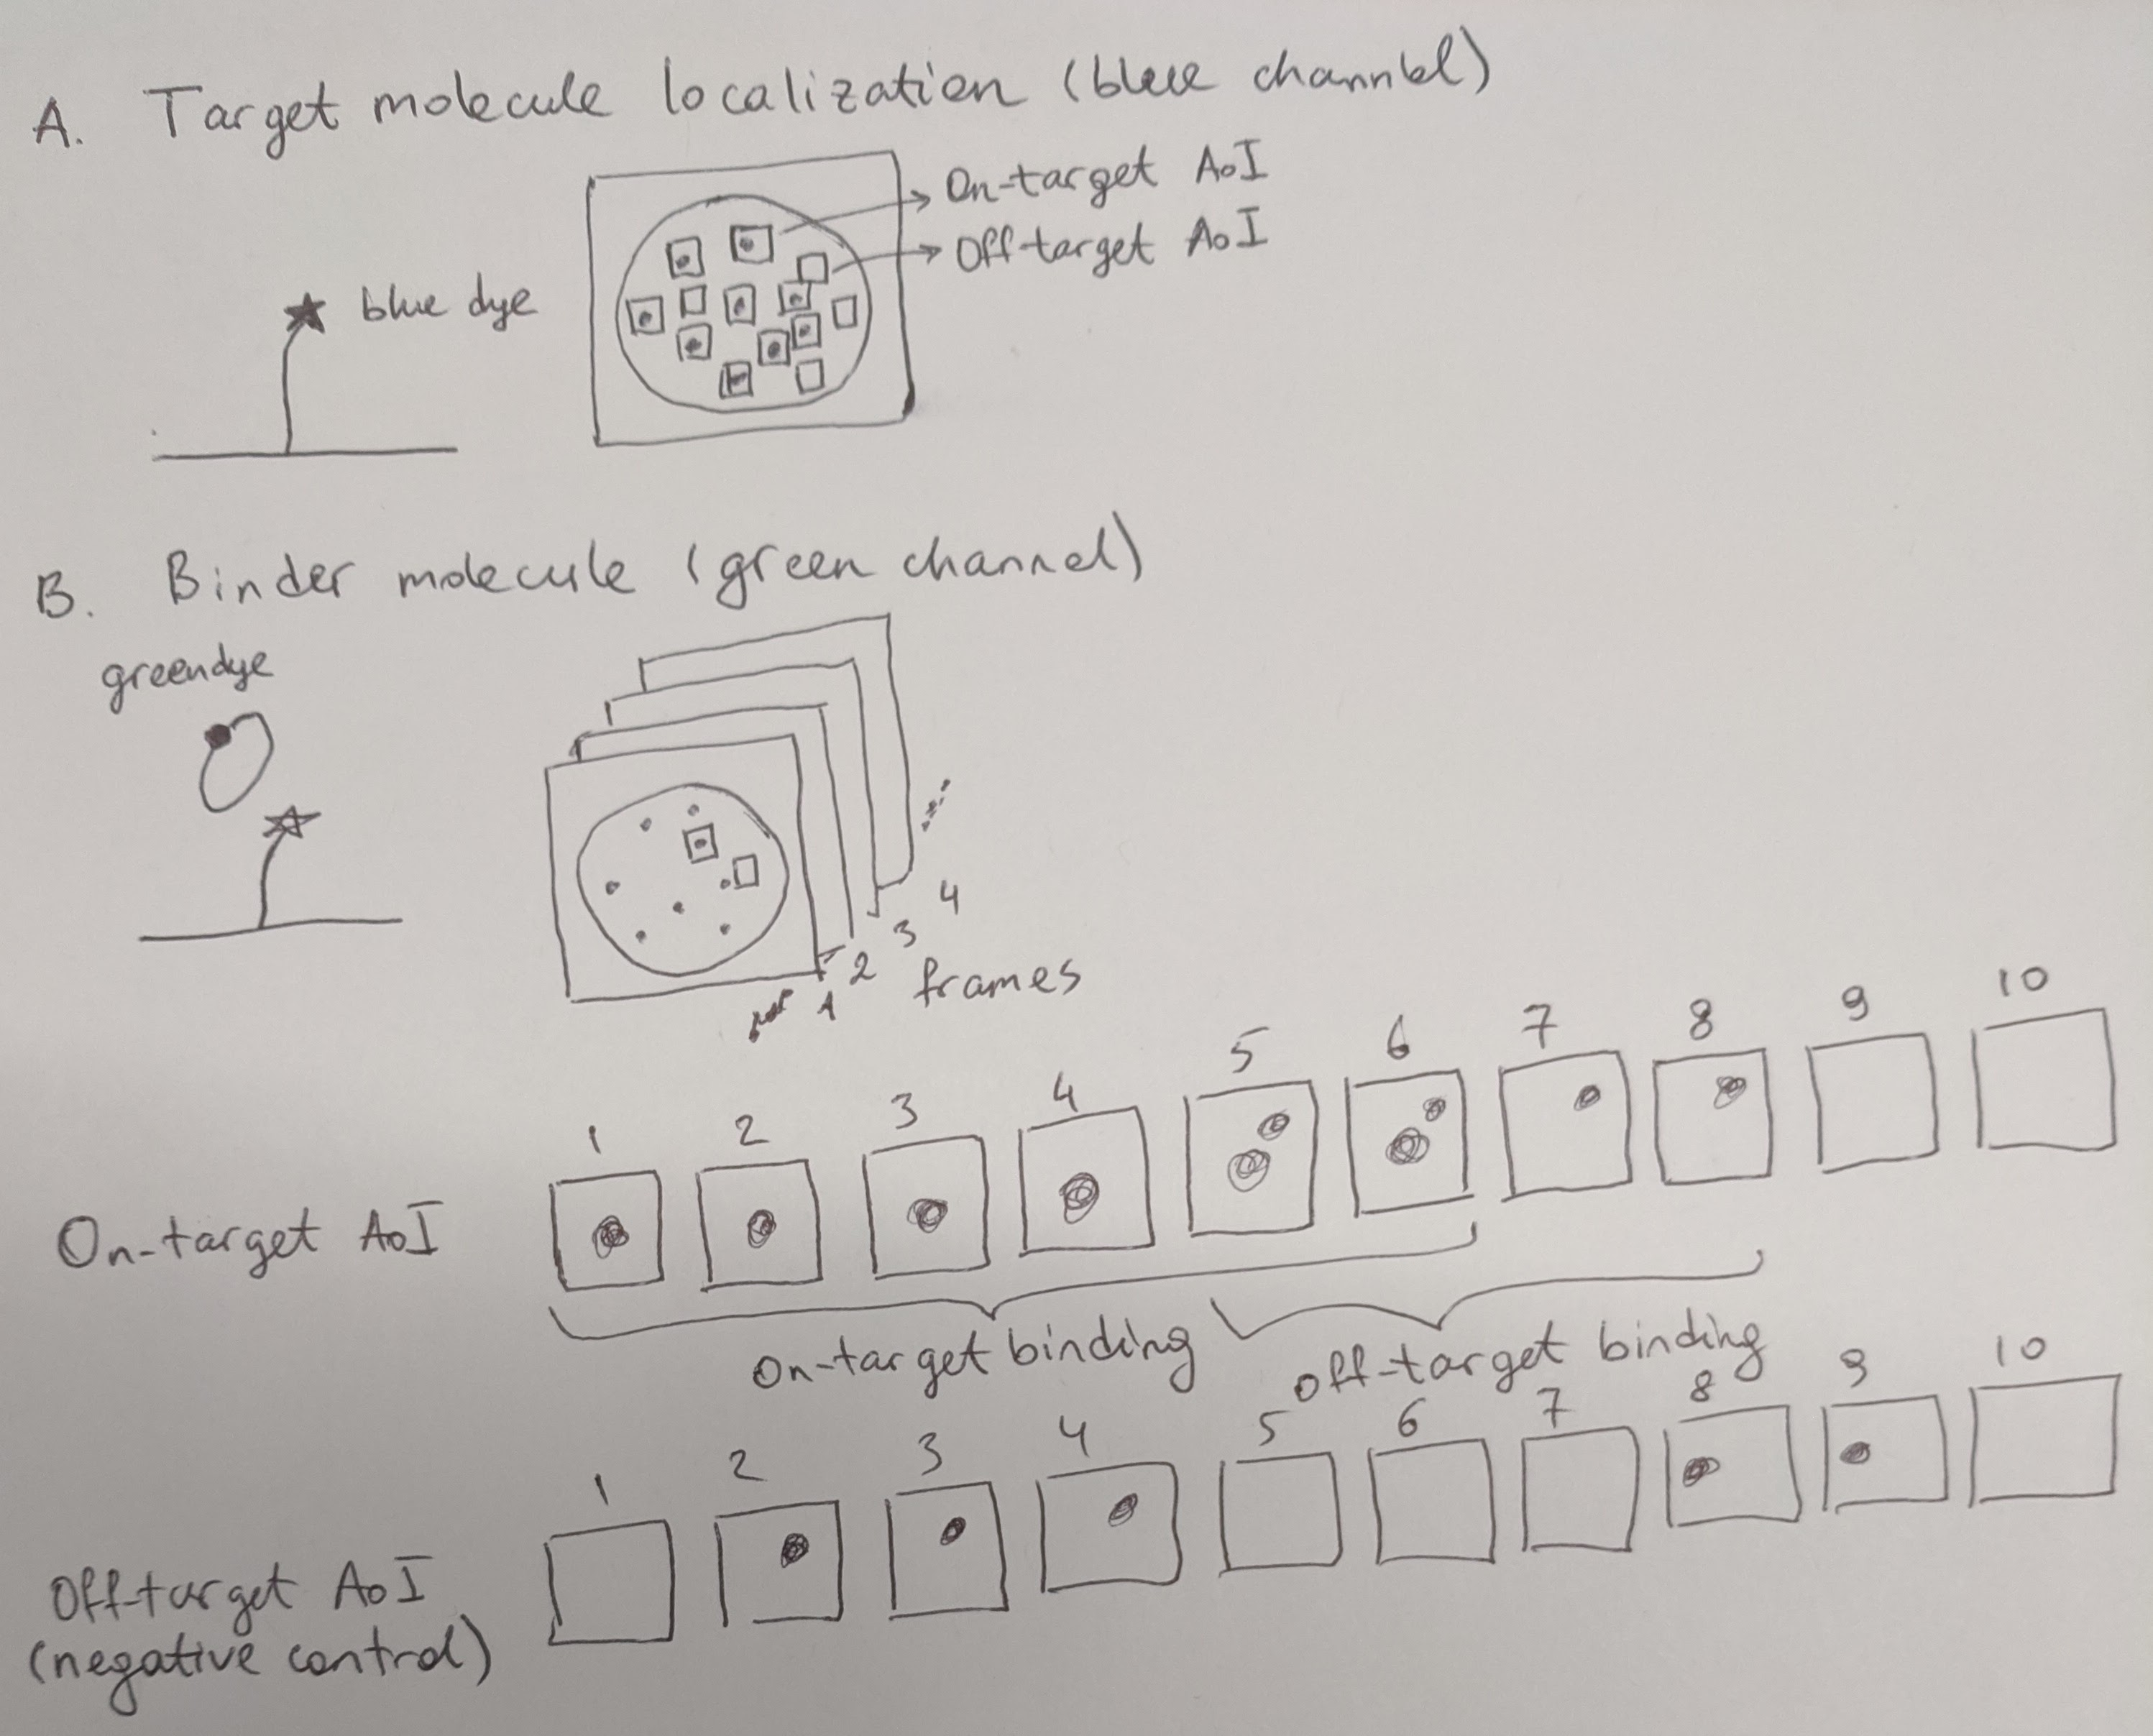
\includegraphics[width=\linewidth]{figures/figure1.jpg}
%\caption{Co-localization single molecule spectroscopy experiment. (A) Target molecules are localized in the blue channel and then on-target and off-target areas of interest are selected. (B) Movies of the binder molecule collected in the green channel. In selected AoI binder molecules can be on-target, off-target, or absent.}
%\label{fig:cosmos_experiment}
%% If the optional argument in the square brackets is "none", then the caption *will not appear in the main figure at all* and only the full caption will appear under the supplementary figure at the end of the manuscript.
%\figsupp[Shorter caption for main text.]{This is a supplementary figure's full caption, which will be used at the end of the manuscript.}{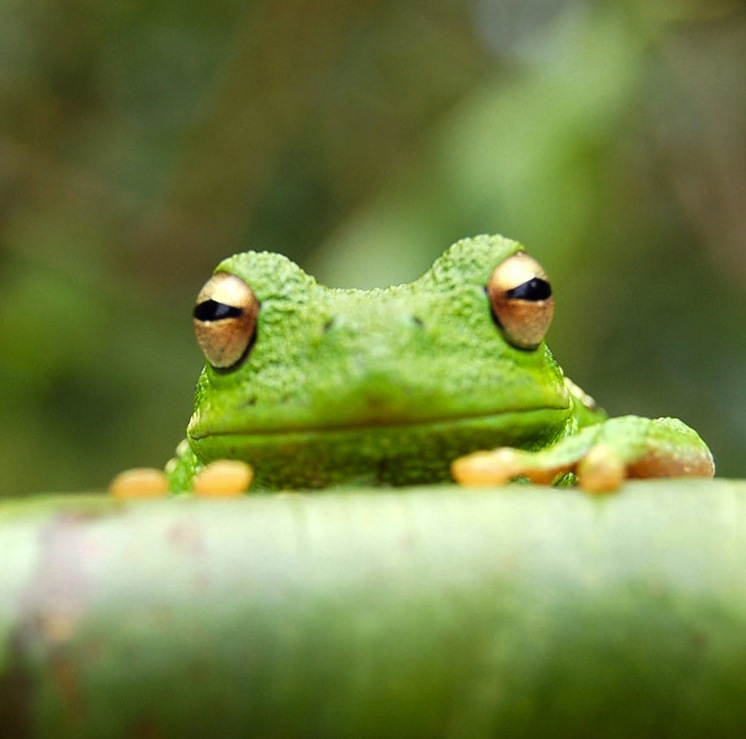
\includegraphics[width=6cm]{frog}}\label{figsupp:sf1}
%\figsupp{This is another supplementary figure.}{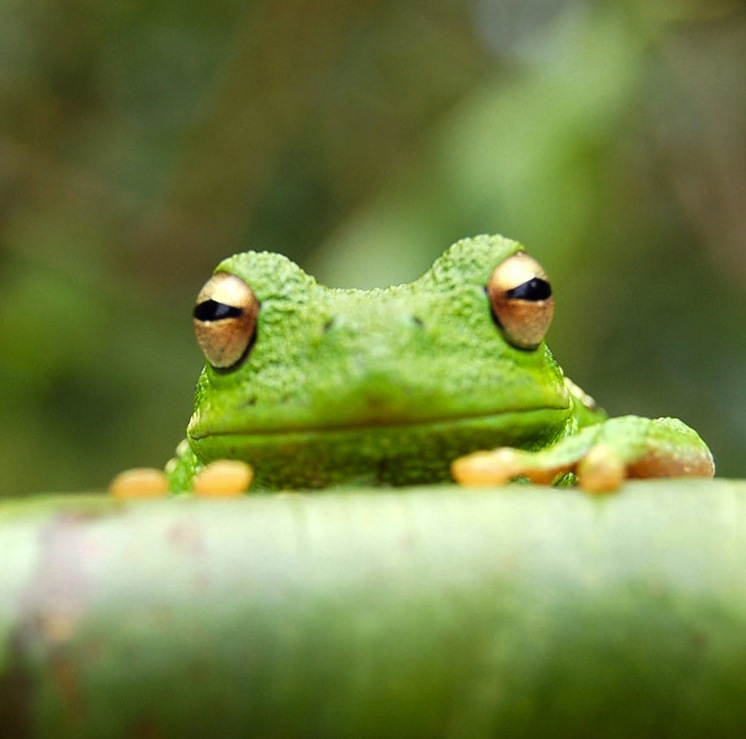
\includegraphics[width=6cm]{frog}}
%\figdata{This is a description of a data source.}\label{figdata:first}
%\figdata{This is another description of a data source.}\label{figdata:second}
%\end{figure}

%\begin{figure}
%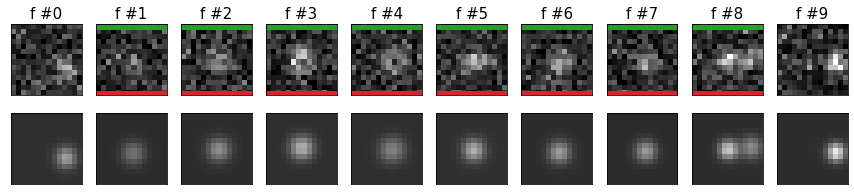
\includegraphics[width=\linewidth]{figures/figure3a.png}
%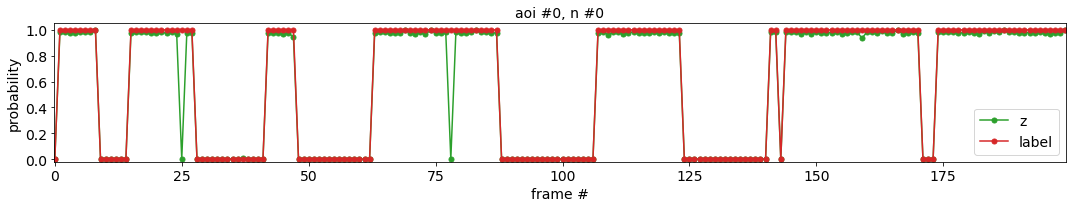
\includegraphics[width=\linewidth]{figures/figure3b.png}
%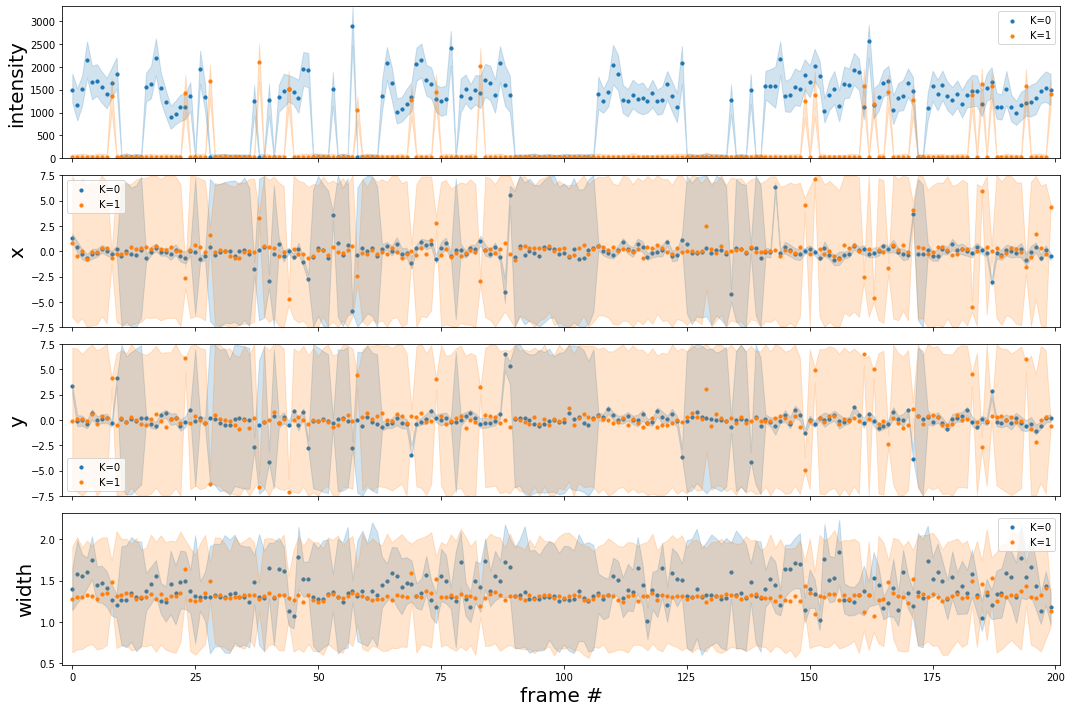
\includegraphics[width=\linewidth]{figures/figure3c.png}
%\caption{Co-localization single molecule spectroscopy experiment. (A) Target molecules are localized in the blue channel and then on-target and off-target areas of interest are selected. (B) Movies of the binder molecule collected in the green channel. In selected AoI binder molecules can be on-target, off-target, or absent.}
%\label{fig:view}
%\end{figure}